\documentclass{article}
\usepackage{ctex}
\usepackage{hyperref}
\usepackage{geometry}
\usepackage{amsmath}
\usepackage{caption}
\RequirePackage{longtable,multirow,array}
\RequirePackage{booktabs}
\usepackage{booktabs}
\usepackage{multicol}
\usepackage{longtable}
\usepackage{booktabs}
\usepackage{algorithm}
\usepackage{algpseudocode}
\usepackage[style=ieee,sorting=nyt]{biblatex}
\assignrefcontextentries[]{*}
\addbibresource{References.bib}
\geometry{left=1in, right=1in, top=1in, bottom=1in}
\hypersetup{hidelinks}
\hypersetup{bookmarksnumbered=true,
	bookmarksopen=true,
	colorlinks=true,
	linkcolor=black,
	citecolor=blue,
	urlcolor=black}
\usepackage{tikz}
\usepackage{pgfplots}
\usepackage{mhchem}
\pgfplotsset{compat=1.18}
\captionsetup{justification=centering}
\captionsetup[figure]{name={Fig.},labelsep=space,labelfont=bf}
\captionsetup[table]{name={Table},labelsep=space,labelfont=bf}
\CTEXoptions[today=old, contentsname=Contents]
\newcommand{\authyear}[1]{\citeauthor{#1} (\citeyear{#1})}
\setmainfont{Arial}

\newcommand{\toB}[1]{\color{blue}#1\color{black}}

\begin{document}
	\title{\vspace{-2.25cm} Development of Ocular Disease Auxiliary Diagnosis System}
	\author{Jerry Pan}
	\date{}
	\maketitle
	
	\vspace{0.5cm}
	\tableofcontents
	
	\pagebreak
	
	\section{Background}
		
		Ocular diseases can be diagnosed through various methods, including using optical coherence tomography (OCT) and color fundus images. Ophthalmologists usually identify ocular abnormalities to deduce the disease.  Traditionally, the diagnosis primarily depends on the professional experience and knowledge of the ophthalmologists, which may result in high misdiagnosis rate and under-utilization of medical data.  With the widespread application of artificial intelligence (AI), deep learning (DL) has made great contributions in providing support to patients in remote areas by sharing expert knowledge \autocite{Ichhpujani_Thakur_2021}.  By leveraging DL, researchers have developed auxiliary diagnosis programs to help doctors in the process. Many studies use convolutional neural network (CNN) to analyze ocular images. Some commonly used CNNs are VGG16, ResNet50, and Inception \autocite{daich2023artificial}.  And for segmenting images and finding abnormalities, U-net is widely used \autocite{Ronneberger_Fischer_Brox_2015}. In training CNNs, most studies use transferred learning, which consists of three steps: learning, fine-tuning, and validation.
		
		Some studies directly predict the disease from OCT images.
		\authyear{li2019deep} used ResNet to analyze OCT images and distinguish between choroidal neovascularization (CNV), diabetic macular edema (DME), drusen, and normal eyes. In addition, they performed occlusion testing to find out the regions that are the most important in diagnosis \autocite{li2019deep}. 
		\authyear{yoo2021feasibility} used generative adversarial network (GAN) and Inception-v3 together with a few-shot dataset to investigate the feasibility of improving OCT diagnosis of rare ocular diseases \autocite{yoo2021feasibility}.  They cleverly handled the issues of training image shortage and data imbalance by creating ocular disease OCT images from healthy OCT images. \authyear{Kermany2018} conducts medical diagnosis and identifies treatable diseases by image-based deep learning.  They also provided a widely used database including more than one hundred thousand OCT labeled images for 3 diseases \autocite{Kermany2018}.
		
		Some other studies can identify ocular abnormalities from annotated OCT images.
		\authyear{camino2018deep} used DL to identify the region of preserved photoreceptors on \textit{en face} OCT in choroideremia and retinitis pigmentosa (RP) \autocite{camino2018deep}. 
		\authyear{srinivasan2014fully} detected DME and dry age-related macular degeneration (dry AMD) from OCT images by flattening the image and using support vector machine (SVM) to extract the thickness information of the retinal layers \autocite{srinivasan2014fully}. 
		\authyear{leandro2023oct} implemented VGG to identify up to 8 kinds of key abnormalities and hence detect multiple diseases by using central fovea cross-section OCT \autocite{leandro2023oct}.  \authyear{Fang_Wang2019} developed a novel lesion-aware CNN, called LACNN, to simulate the ophthalmologists' diagnosis that focuses on ocular abnormalities.  The LACNN is a U-net-like CNN which incorporates VGG16 as the baseline, and the result is impressive \autocite{Fang_Wang2019}.
		
		Other studies use fundus images to predict ocular diseases.
		\authyear{masumoto2019accuracy} trained deep CNN with ultrawide-field fundus images to make the CNN capable of diagnosing RP \autocite{masumoto2019accuracy}. 
		\authyear{chen2021artificial} uses color fundus photographs and multiple types of CNN (Inception V3, Inception Resnet V2, and Xception) to develop a method of early detection of RP \autocite{chen2021artificial}. 
		\authyear{li2022development} uses CNN to detect up to 12 fundus diseases based on colour fundus photography \autocite{li2022development}.  \authyear{Son2023} presented a novel architectural and algorithmic design to comprehensively identify 15 abnormalities and diagnose 8 major ocular diseases from macula-centered fundus images.  They defined a notion of counterfactual attribution ratio (CAR) to interpret the system's diagnostic reason and disclose the relationship between abnormalities and diseases \autocite{Son2023}.
		
		In recent years, more and more DL systems began to use multi-modal information to predict ocular diseases.  For automated detection system, retrieving features from both OCT images and fundus images can effectively keep the diagnosis away from bias and incompleteness.  It is not always necessary to yield a better automated diagnosis result, but it does help ophthalmologist to make more accurate and holistic clinical decisions.  For instance, \authyear{liu2023prediction} combined OCT and fundus images to evaluate visual impairment in RP in terms of best-corrected visual acuity(BCVA) \autocite{liu2023prediction}.  \authyear{Xu2021} leveraged a bi-modal CNN to diagnose AMD and polypoidal choroidal vasculopathy (PCV), where the architecture uses fundus and OCT images as input for transferred learning CNN and concatenates the retrieved features to classify 3 diseases including dry AMD, wet AMD and PCV \autocite{Xu2021}.  And \author{Andrearczyk2018} ingeniously combined medical images and biomedical textual information to discriminate different diseases, which is a novel method for the usage of multi-modal application \autocite{Andrearczyk2018}.
		
		The key technical problem of multi-modal diagnosis is how to fuse the results from multifarious sources.  There are three types of fusion, namely early, late, and hybrid fusion.  Deciding on the optimal type of fusion is part of the exploratory process in the application of DL methods \autocite{Ichhpujani_Thakur_2021}.
		
		
	\section{Purpose}
		
		We will develop an Ocular Disease Auxiliary Diagnosis System (ODADS). 
		
		\vspace{0.3cm}
		
		\textbf{First, the ODADS aims to simulate the comprehensive diagnosis process by considering information from both fundus and OCT images.} While both types of images can respectively indicate different diseases, they can also strengthen certain disease discrimination.  Considering both sources can result in a more comprehensive disease diagnosis.
		
		\vspace{0.1cm}
		
		\textbf{Second, the ODADS aims to present more interpretable findings.}  Most studies provide end-to-end systems for classifying diseases as black boxes, which may not be convincing enough when their results are different from ophthalmologists'.  The ODADS will provide 2 types of results, namely abnormalities and disease.  We will highlight all the abnormalities and use them to deduce diseases, so that the ODADS could provide as much information as possible.  Even when the ODADS does not automate diagnosis correctly, the results can still be references for users.
		
		\vspace{0.1cm}
		
		\textbf{Third, the ODADS aims to provide the probabilities of ocular diseases.}  Most studies only do the classification, which is not enough in some scenarios.  The symptoms could be complex, where multiple disease could be in the same case.  Providing diseases probabilities than simple discrimination can enable users to be aware of actual ocular conditions and potentially improve treatment.
		
		\vspace{0.1cm}
		
		\textbf{Fourth, The ODADS aims to be accessible to all people.}  While most studies design models dedicated to ophthalmologists, the ODADS will contain a website and a mobile application (APP) to serve people including ophthalmologists, patients and their families, and all others.

		\vspace{0.1cm}

		\textbf{Last, The ODADS aims to be more flexible by allowing user to input multiple images.}  Most studies only consider limited images.  In other words, mono-modal systems only work on one fundus image or one OCT image and bi-modal systems only work on 2 images.  The ODADS will enable user to input more than 2 images, especially for OCT images, which could result in more accurate diagnosis. 
		
	\section{Models}
		
		The ODADS will consist of two parts. 
		
		The first part is a back-end model, which has fundus and OCT images as input and features and probabilities as output. The second part is a front-end user interface (UI), including a website and an APP, which implements the back-end model and provides users with diagnosis information.
		
		The back-end model will be built based on multiple sub-models including several OCT-Models, several Fundus-Models and one Diagnosis-Model.  Each OCT-Model and Fundus-Model will contain a classifier which will be trained separately by a backboned ResNet50.  Diagnosis-Model will consist of a neural network for determining the deduction from abnormalities to diseases.  We will study the optimal OCT-Model and Fundus-Model number and compare different fusion timing to determine the best architecture.  The back-end model will output 2 sets of results to the front-end UI, one containing the probabilities of potential ocular diseases and the other containing abnormalities and their locations in each image.
		
		The front-end UI will enable users to upload OCT and fundus images, which can be got by taking photos in the APP or selecting image files from disk on the website. The UI will generate a report, including the ocular abnormalities, their locations, and the probabilities of different ocular diseases, etc. Ophthalmologists can use the APP or website to assist their diagnosis. And if patients and their families can get their OCT and fundus images from the hospital, they can also use the UI to view the report, which can be a supplementary reference to clinical diagnosis.  The front-end UI will also provide some functionalities like viewing the locations of abnormalities interactively and revising the automated diagnosis results of diseases and abnormalities and upload the revision to server for improving the back-end model in the future.
	
	\pagebreak
	\section{Abnormalities and Diseases} \label{sec:ab_di}
	
	\subsection{OCT Abnormalities}
	
		Fig.\ref{fig:oct-abnormalities} shows the OCT abnormalities in the ODADS.
		Table \ref{tb:oct-abnormalites} lists the description of abnormalities.
		
		{
			\fontsize{9}{12}\selectfont
			{
				\begin{longtable}{lp{3.8in}}
				\caption{OCT Abnormalities}
				\label{tb:oct-abnormalites}\\
				\toprule
				Abnormality&Description\\
				\toprule
				
				\multicolumn{1}{l}{Central serous chorioretinopathy (CSC)}
				& \multicolumn{1}{l}{The accumulation of fluid underneath the retina.}\\
				
				\multicolumn{1}{l}{Epiretinal membrane (ERM)}
				& A thin layer of fibrous tissue forms on the surface of the retina, particularly the macula.\\
				
				\multicolumn{1}{l}{Macular hole (MH)}
				& Disruption or discontinuity in the normal retinal layers surrounding the macular hole.\\
				
				\multicolumn{1}{l}{Retinal detachment}
				& The separation between the neurosensory retina and the underlying retinal pigment epithelium (RPE) or choroid.\\

				\multicolumn{1}{l}{Stargardt disease}
				& Thinning and atrophy of the retina. Disruption of photoreceptor layers. Presence of subretinal deposits.\\

				\multicolumn{1}{l}{Retinitis pigmentosa (RP)}
				& Thinning of the Retinal Layers. Disruption of Photoreceptor Layers. Attenuation of Retinal Vasculature.\\

				\multicolumn{1}{l}{Macular telangiectasia (Mactel)}
				& Abnormalities in the macular blood vessels, leading to changes in the macular structure and function\\

				\multicolumn{1}{l}{Diabetic macular edema (DME)}
				& The accumulation of fluid in the macula. \\

				\multicolumn{1}{l}{Macular neovascularization}
				& The abnormal growth of new blood vessels in the macular region of the retina.\\

				\multicolumn{1}{l}{Subretinal fluid}
				&  The accumulation of fluid between the neurosensory retina and the retinal pigment epithelium (RPE)\\

				\multicolumn{1}{l}{Intraretinal fluid}
				& The accumulation of fluid within the layers of the retina.\\
				
				\multicolumn{1}{l}{Drusen}
				& Small deposits of extracellular material that accumulate beneath the retinal pigment epithelium (RPE) or between the RPE and the photoreceptor layer in the macular region of the retina.\\

				\bottomrule
				\end{longtable}
			}
		}
	
	\subsection{Fundus Abnormalities}
	
	Fig.\ref{fig:fundus-abnormalities} shows the fundus abnormalities in the ODADS.
	Table \ref{tb:fundus-ab} lists the description of abnormalities.
	
	{
		\fontsize{9}{12}\selectfont
		{
			\begin{longtable}{lp{3.8in}}
				\caption{Fundus Abnormalities}
				\label{tb:fundus-ab}\\
				\toprule
				Abnormality&Description\\
				\toprule
				
				\multicolumn{1}{l}{Epiretinal membrane (ERM)}
				& Retinal Wrinkling.  Foveal Reflex Changes. Retinal Vessel Distortion\\
				
				\multicolumn{1}{l}{Macular hole (MH)} & Full-thickness macular hole showing a surrounding cuff of subretinal fluid.\\
				
				\multicolumn{1}{l}{Retinal nerve fiber layer defect} & A dark stripe or wedge-shaped localized defect in the peripapillary area, parallel to the normal retinal striation, or as a diffuse loss of this striation. \\
				
				\multicolumn{1}{l}{Glaucomatous disc change} & Cupping.  Cup-to-Disc Asymmetry. Thinning of Neuroretinal Rim. Optic Nerve Head Hemorrhages \\
				
				\multicolumn{1}{l}{Hard exudate} & Yellow or Yellow-White Deposits.  Hard Borders.  Distribution.  Clustering Around Blood Vessels\\
				
				\multicolumn{1}{l}{Hemorrhage} & Small dot-like to larger blot.  Fresh hemorrhages typically appear bright red or deep red in color, indicating the presence of oxygenated blood. Over time, as the blood undergoes degradation and clotting, the hemorrhage may change color to darker red, orange, or yellowish hues.\\
				
				\multicolumn{1}{l}{Cotton wool patch / soft exudate} & White or off-white lesions.  Irregular shapes and margins.\\
				
				\multicolumn{1}{l}{Fluid accumulation} &  a localized or diffuse elevation of the retina, often with a smooth or dome-shaped contour\\
				
				\multicolumn{1}{l}{Vascular abnormality} & Retinal Vessel Tortuosity.  Retinal Vessel Caliber Changes.  \\
				
				\multicolumn{1}{l}{Choroidal lesion} & Flat, well-defined areas of pigmentation ranging from light brown to dark brown. \\
				
				\multicolumn{1}{l}{Drusen} & Small, round or oval-shaped yellow or white deposits.\\
																
				\bottomrule
			\end{longtable}
		}
	}
	
	\begin{figure}[htbp]
		\centering
		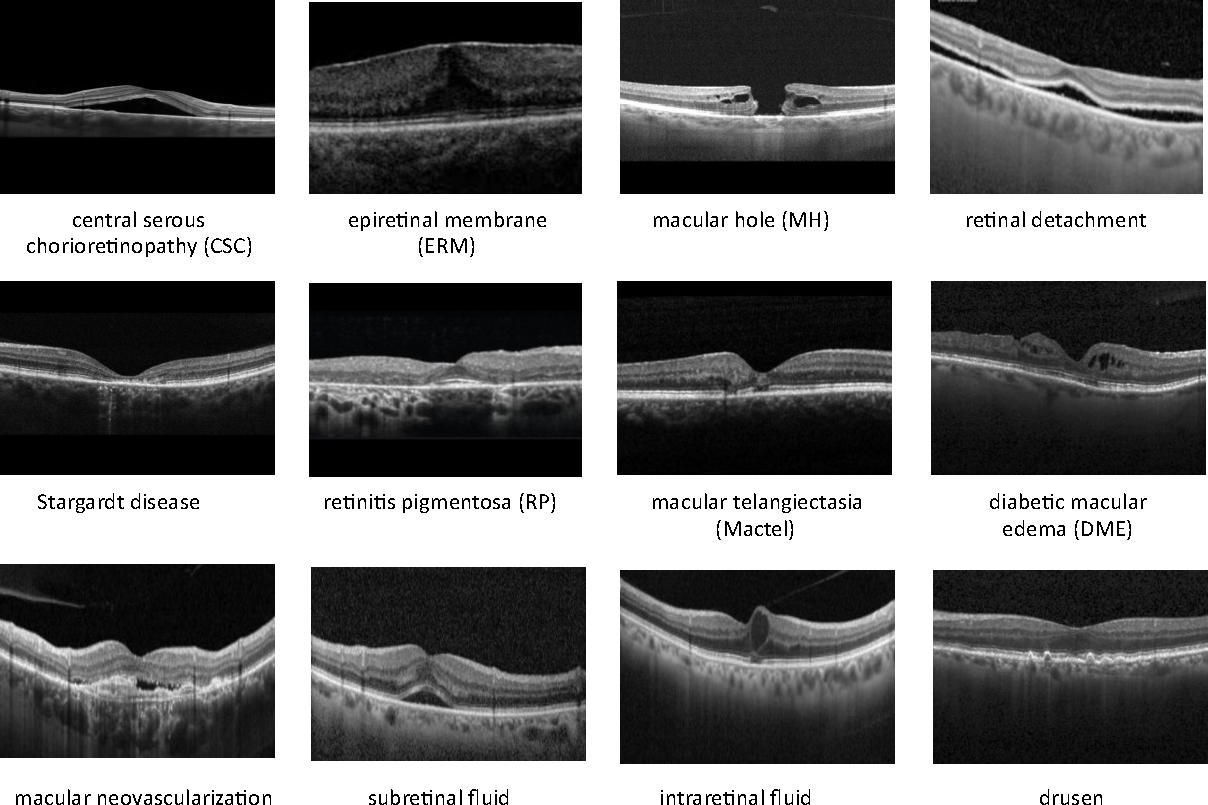
\includegraphics[width=0.9\linewidth]{OCT-abnormalities.pdf}
		\caption{OCT Abnormalities}
		\vspace{0.3cm}
		\label{fig:oct-abnormalities}
	\end{figure}
	
	\begin{figure}[htbp]
		\centering
		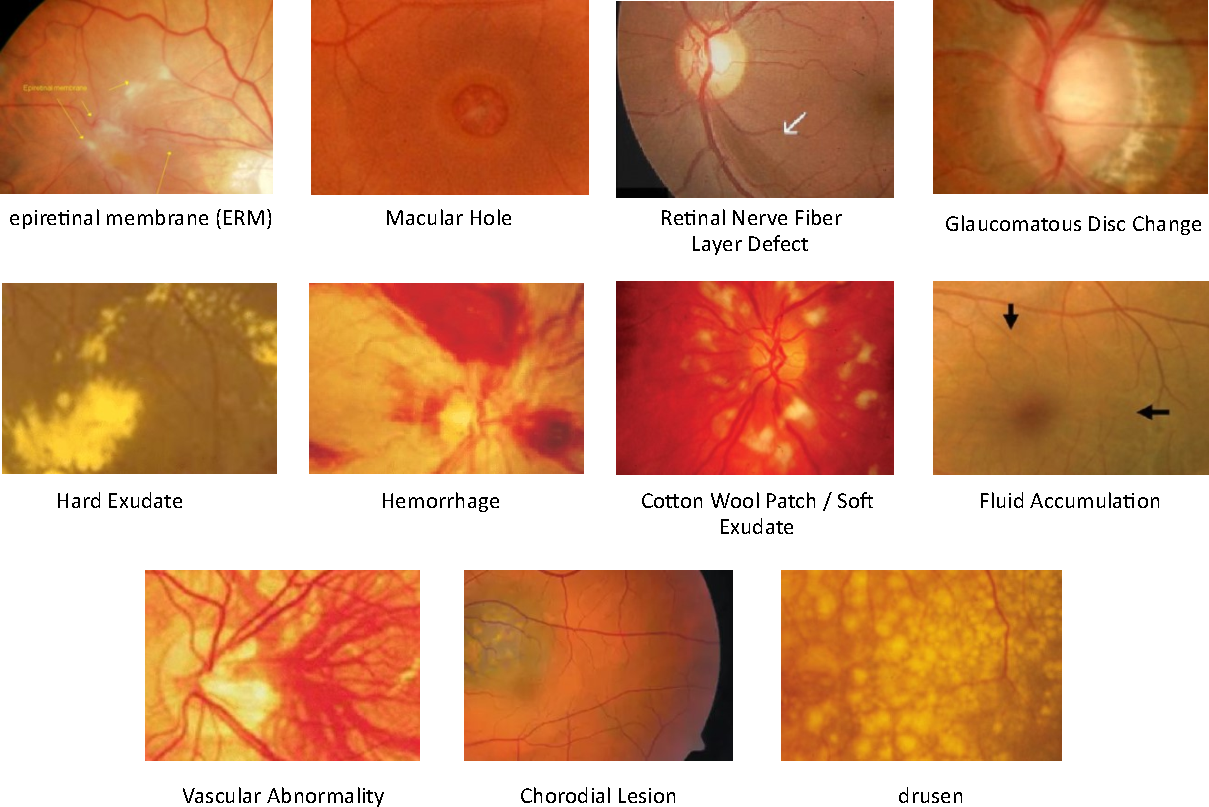
\includegraphics[width=0.9\linewidth]{fundus-ab.pdf}
		\caption{Fundus Abnormalities}
		\vspace{0.3cm}
		\label{fig:fundus-abnormalities}
	\end{figure}
	
	\subsection{Diseases}
		Table \ref{tb:diseases} lists the diseases in ODADS.
	
		{
		\fontsize{9}{12}\selectfont
		{
			\begin{longtable}{lp{3.8in}}
				\caption{Diseases}
				\label{tb:diseases}\\
				\toprule
				Abnormality&Description\\
				\toprule
				
				\multicolumn{1}{l}{Central Serous Chorioretinopathy} & The accumulation of fluid under the retina, specifically in the macular region, leading to vision disturbances.\\
				
				\multicolumn{1}{l}{Epiretinal Membrane} & Also known as macular pucker or cellophane maculopathy, a condition characterized by the formation of a thin, semitransparent membrane on the surface of the retina, particularly in the macular region. Here's an overview of epiretinal membrane. \\
				
				\multicolumn{1}{l}{Macular Hole} & A defect or opening in the center of the macula, the central part of the retina responsible for sharp central vision. \\
				
				\multicolumn{1}{l}{Glaucoma Suspect} & Exhibit one or more risk factors or suspicious findings that suggest they may be at increased risk of developing glaucoma in the future. \\
				
				\multicolumn{1}{l}{Retinal Detachment} & The retina, the light-sensitive tissue lining the back of the eye, becomes separated from its underlying layers of support\\
				
				\multicolumn{1}{l}{Stargardt Disease} & Also known as Stargardt macular dystrophy or fundus flavimaculatus, is a genetic eye disorder characterized by progressive degeneration of the macula, the central part of the retina responsible for sharp central vision.\\
				
				\multicolumn{1}{l}{Mild DR} & Mild diabetic retinopathy (DR) refers to the early stages of retinal damage caused by diabetes. \\
				
				\multicolumn{1}{l}{Referable DR} & Referable diabetic retinopathy (DR) refers to the presence of diabetic retinopathy that requires referral to an ophthalmologist or retina specialist for further evaluation and management. This designation typically applies to cases of moderate to severe diabetic retinopathy or the presence of sight-threatening complications such as diabetic macular edema (DME). \\
				
				\multicolumn{1}{l}{Dry AMD} & Dry age-related macular degeneration (AMD) is characterized by the gradual deterioration of the macula due to the accumulation of drusen (yellowish deposits) and the loss of retinal pigment epithelial (RPE) cells, photoreceptors, and other retinal cells. It is the most common form of AMD, accounting for approximately 85-90\% of all cases.\\
				
				\multicolumn{1}{l}{Wet AMD} & Wet AMD is a more severe form of AMD compared to dry AMD. It is characterized by the growth of abnormal blood vessels (choroidal neovascularization) beneath the macula. These blood vessels are fragile and leak fluid and blood, causing damage to the macula and leading to rapid vision loss if left untreated.\\
				
				\multicolumn{1}{l}{BRVO / HCRVO} & Branch retinal vein occlusion (BRVO) and hemiretinal vein occlusion (HCRVO) are two types of retinal vein occlusion, which occur when one or more of the veins that carry blood away from the retina become blocked or occluded.\\
				
				\multicolumn{1}{l}{CRVO} & Central retinal vein occlusion (CRVO) is a serious eye condition that occurs when the main vein that drains blood from the retina becomes blocked or occluded. This blockage leads to a buildup of pressure in the retinal veins, causing hemorrhages, edema (fluid buildup), and ischemia (lack of blood flow) in the retina. \\
				
				\multicolumn{1}{l}{Retinitis Pigmentosa (RP)} & Retinitis pigmentosa (RP) is a group of inherited retinal disorders characterized by progressive degeneration of the retina, leading to vision loss and, in severe cases, blindness. RP typically affects the rod and cone photoreceptor cells in the retina, which are essential for vision in low light (rods) and daylight and color vision (cones). \\
				
				\multicolumn{1}{l}{Macular Telangiectasia (Mactel)} & 
				Macular telangiectasia, also known as idiopathic juxtafoveal retinal telangiectasis (IJRT) or idiopathic macular telangiectasia (IMT), is a rare, progressive eye condition characterized by abnormal dilation and leakage of blood vessels in the macula, the central part of the retina responsible for sharp central vision. Macular telangiectasia primarily affects the retinal capillaries in the juxtafoveal region, leading to vision loss and, in severe cases, legal blindness.\\
				
				\bottomrule
			\end{longtable}
		}
	}
	
	\section{Back-end Model}
	
		The back-end model is shown in Fig.\ref{fig:back-end}.  
		
		The model contains $n$ OCT-Models, $m$ Fundus-Models and one Diagnosis Model.  The OCT-Models and Fundus-Models are fed by OCT images and fundus images respectively, and output image features and abnormality probabilities to the Diagnosis-Model where the data is fused and calculated.  Ultimately the diagnosis result is generated and outputted to Front-end UI.

		\vspace{0.5cm}

		\begin{figure}[htbp]
			\centering
			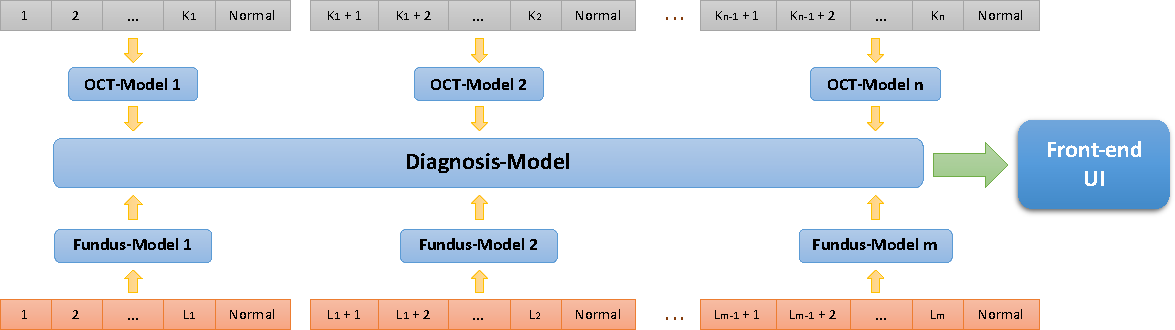
\includegraphics[width=\linewidth]{Back-end.pdf}
			\caption{Back-end Model}
			\label{fig:back-end}
		\end{figure}
		
	\subsection{Classifier}
		Each OCT-Model and Fundus-Model uses several types of abnormalities with the normal for training, which makes the model a classifier in the ODADS, as shown in Fig.\ref{fig:back-end}. 
		
		We have the following formulas.

		\[
		N = \sum_{i=1}^{n} K_i \qquad M = \sum_{i=1}^{m} L_i
		\]
		
		Where:
		
		$n$: the OCT-Model number.
		
		$m$: the Fundus-Model number.
		
		$K_i$: the classifying abnormality number in $i^{th}$ OCT-Model.
		
		$L_i$: the classifying abnormality number in $i^{th}$ fundus-Model.
		
		$N$: the total abnormality number in OCT images.
		
		$M$: the total abnormality number in fundus images.
		
		\vspace{0.3cm}		
		We use the Greedy Algorithm to determining $K_i$, $L_i$, $n$, and $m$.
		
		Fig.\ref{fig:classifier} is an example to illustrate how OCT-Model 1 is generated.  First we choose the first abnormality and the normal to assemble a bi-classifier and calculate its performance (We will use F1-score as the performance indicator, refer to Section \ref{sec:results} for more information).  Then we introduce the second abnormality to form a new tri-classifier including 2 abnormalities and the normal.  If the performance of tri-classifier is better than the bi-classifier, we adopt the tri-classifier, otherwise we still use bi-classifier.  All the abnormalities are introduced in turn, either adopted or abandoned by the OCT-Model 1, and finally we get the classifier for OCT-Model1 including $K_i$ abnormalities and the normal.  Then we generate other classifiers in the same way as the first one until all the abnormalities belong to specific classifiers.

		\vspace{0.5cm}

		\begin{figure}[htbp]
			\centering
			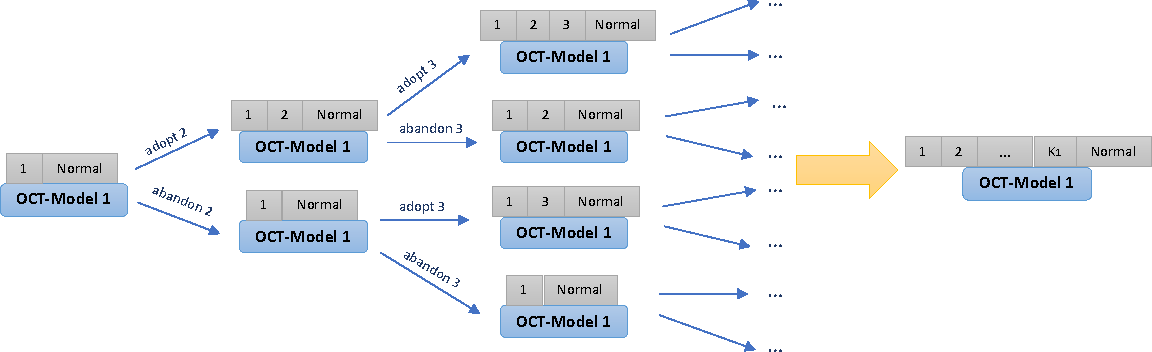
\includegraphics[width=\linewidth]{Classifier.pdf}
			\caption{Classifiers Generation Algorithm}
			\label{fig:classifier}
		\end{figure}

		\vspace{0.5cm}	
		
		We will set up a threshold for performance comparison.  Even when one classifier with more abnormalities has lower performance than another classifier with less abnormalities but the gap is within the threshold, we still choose the classifier with more abnormalities because we need to minimum classifier number to insure smaller CNN parameter quantities, faster running and easier deployment.
				
	\subsection{OCT-Model and Fundus-Model}
		The OCT-Model and fundus-Model use ResNet50 as backbones.  We apply transferred learning to train the ResNet50, which includes 2 phases, namely taking the models with the parameters learned with ImageNet and then performing a fine-tuning process.  
		
		Fig.\ref{fig:resnet50} shows the architecture of OCT-Model and Fundus-Model.  We apply a modified ResNet50 and then flatten the data.  With a full-connected (FC) hidden layer, we get feature vector.  Then with another FC layer, we get abnormalities probabilities.  In Diagnosis-Model, we will determine to use whether feature vector or abnormalities probabilities for data fusion.
		
		\vspace{0.5cm}		
		
		\begin{figure}[htbp]
			\centering
			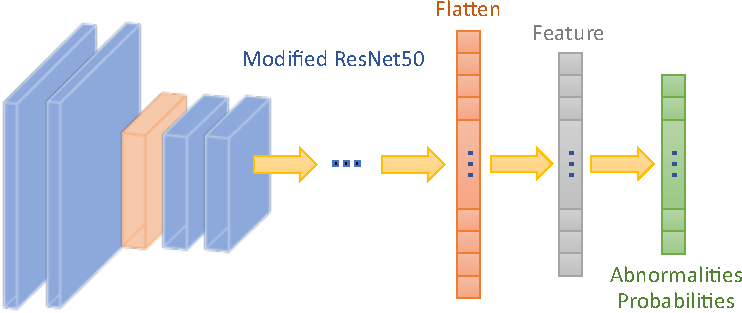
\includegraphics[width=0.6\linewidth]{ResNet50.pdf}
			\caption{OCT-Model and Fundus-Model Architecture}
			\label{fig:resnet50}
		\end{figure}
	
	\subsection{Diagnosis-Model}
		
		The Diagnosis-Model is a neural network which fuses data from OCT-Models and Fundus-Models and then leverages a FC hidden layer to translate abnormalities to diseases.
		Fig.\ref{fig:diagnosis-model} shows 2 solutions for data fusion.  One is to fuse the feature vectors from OCT-Models and fundus-models, and the other is to fuse the probability vectors from those sub-models.  We compare the performance between 2 solutions and choose the better one as our ultimate architecture.
		When we fuse the feature vectors, we concatenate them as a big vector.  And when we fuse the probability vectors, we pick the maximum probability for each abnormality and then normalize the vector to form a new abnormality probability vector.
		
		\vspace{0.5cm}		
		
		\begin{figure}[htbp]
			\centering
			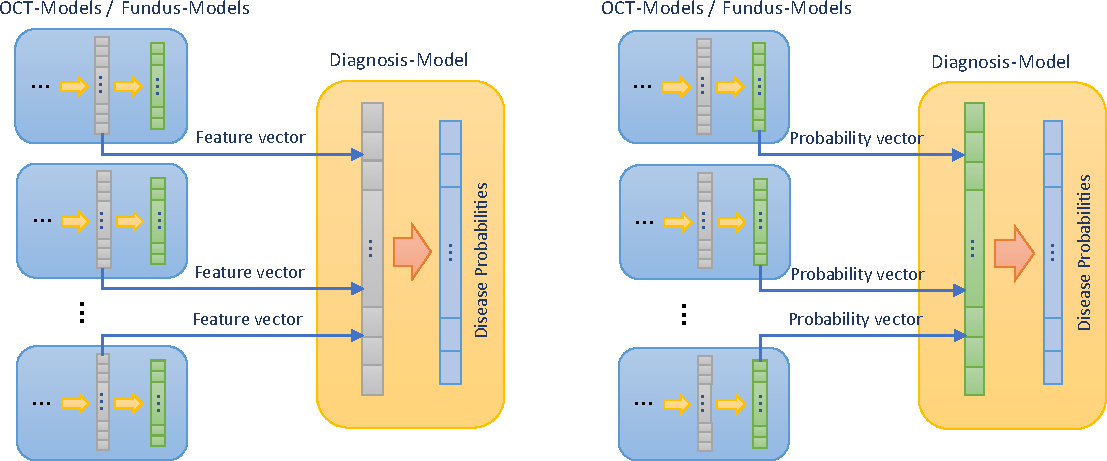
\includegraphics[width=\linewidth]{Diagnosis-Model.pdf}
			\vspace{0.1cm}
			\caption{Diagnosis Model}
			\label{fig:diagnosis-model}
		\end{figure}
		
		For training Diagnosis-Model, we need to set up ground truth in terms of converting abnormalities to diseases.  We refer to 3 books for determining the conversion criteria, namely \textit{\citefield{Wolf_Kirchhof_Reim_2006}{title}}\autocite{Wolf_Kirchhof_Reim_2006}, \textit{\citefield{Duker_Waheed_Goldman_2022}{title}}\autocite{Duker_Waheed_Goldman_2022} and \textit{\citefield{Kawasaki_2013}{title}}\autocite{Kawasaki_2013}.  
		
		The conversion criteria is shown in Fig.\ref{fig:abnormality-disease}, where the gray boxes represent OCT abnormalities, orange boxes represent fundus abnormalities, and blue boxes represent diseases.  Refer to Section \ref{sec:ab_di} for more information regarding abnormalities and diseases.
		
		\vspace{0.3cm}
		
		\begin{figure}[htbp]
			\centering
			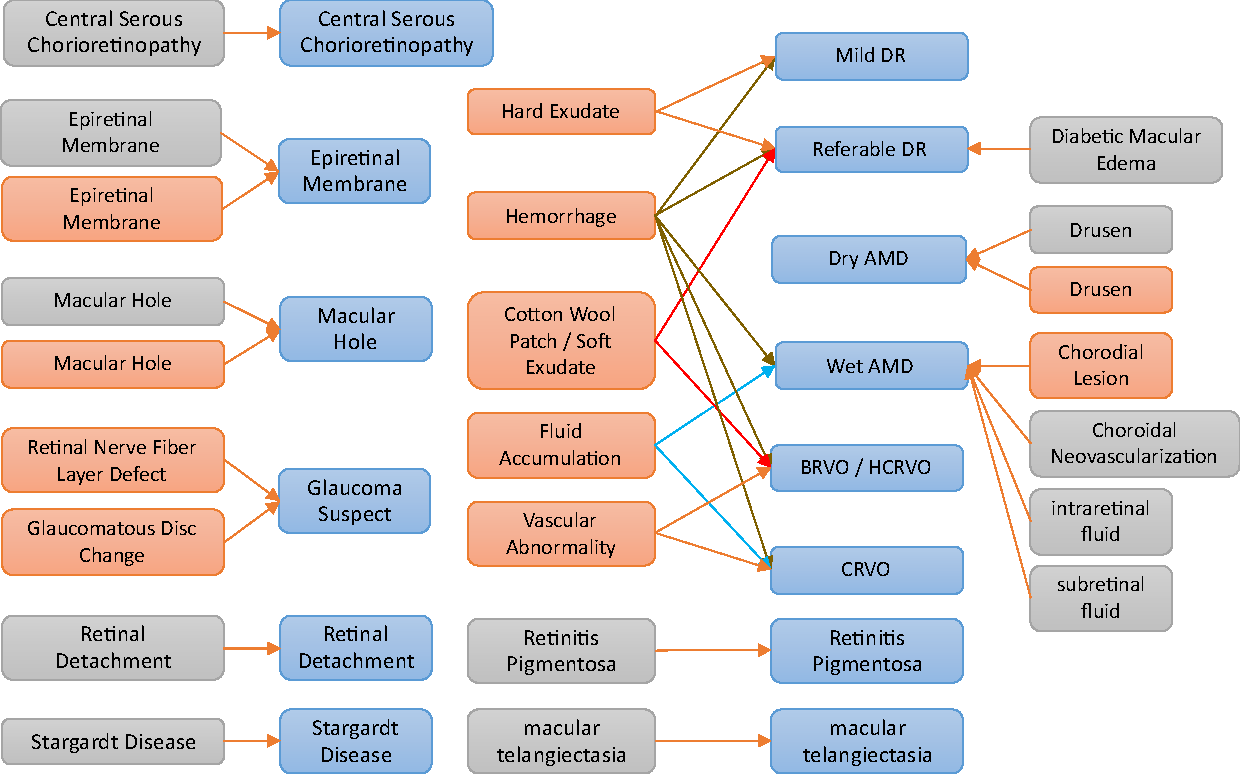
\includegraphics[width=0.95\linewidth]{Abnormality-Disease.pdf}
			\vspace{0.3cm}
			\caption{From Abnormality to Disease}
			\label{fig:abnormality-disease}
		\end{figure}
	
	\subsection{Training}

		We will train all the OCT-Models and Fundus-Models first and determine all the classifiers.  Then we will freeze those models and train the Diagnoal-Model.  The training images will be labeled, prepossessing, augmented when necessary.  The augmentation includes image rotation, translation, scaling, flipping, brightness adjustment, constrat adjust, and noise addition etc.  If training images are too fewer, we will use CycleGAN to generate some synthetic images for training, but we will try to avoid doing this by looking for more public datasets.
		
		The trainings are implemented on a desktop computer with Intel® Xeon® Platinum 8352V Processor, 256G of RAM and 2 NVIDIA GPU (GeForce RTX 4090) with 48 VRAM.
		
		\vspace{0.3cm}
		
		The training images for OCT-Models will come from the following 2 public datasets.
		\begin{enumerate}
			\vspace{-0.2cm}
			\item \textit{Large Dataset of Labeled Optical Coherence Tomography (OCT) and Chest X-Ray Images}\autocite{Kermany_database}.
			\vspace{-0.2cm}
			\item \textit{Data for: Improved accuracy in OCT diagnosis of rare ocular disease using few-shot learning with generative adversarial networks} \autocite{Yoo_2020}.
		\end{enumerate}
		
		\vspace{0.3cm}
		
		The training images for Fundus-Models will come from another 5 public datasets.
		\begin{enumerate}
			\vspace{-0.2cm}
			\item \textit{E-ophtha} \autocite{E_ophtha}.
			\vspace{-0.2cm}
			\item \textit{Diabetic Retinopathy Detection} \autocite{DR_dataset}.
			\vspace{-0.2cm}
			\item \textit{Indian Diabetic Retinopathy Image Dataset. (IDRiD)} \autocite{Porwal_2018}.
			\vspace{-0.2cm}
			\item \textit{Messidor} \autocite{Messidor}.
			\vspace{-0.2cm}
			\item \textit{STructured Analysis of the Retina} \autocite{STARE}.
		\end{enumerate}
		
		\vspace{0.3cm}
		
		We have not found online open dataset for training Diagnosis-Model.  We will need OCT images and fundus images from the same patients.  Online datasets only contain OCT images or fundus images, which do not meet our requirement.
		
		There are 2 plans as follow.  \textcolor{magenta}{We would hope to implement plan A.  Using the real data from hospital could make the ODADS more reliable and robust}.  If plan A is not possible, we will do plan B.
		\vspace{0.1cm}
		\begin{enumerate}
			\vspace{-0.2cm}
			\item \textcolor{magenta}{We will use the data from hospital.  The dataset will contain OCT images and fundus images from patients.  For privacy, we do not need any patient identity information, and each piece of data in the dataset could be organized as "Data Number", "OCT images", "Fundus Images" and "Brief Diagnosis".  This may need to be approved by authorities.}
			\vspace{-0.2cm} 
			\item We will make up the training data on our own.  The image data will come from above public database and the diagnosis will be made by ourselves.
		\end{enumerate}	

	\subsection{Results} \label{sec:results}
	
		We will provide the following performance indicators for each model.
		\vspace{0.1cm}
		\begin{itemize}
			\vspace{-0.2cm}
			\item Confusion Matrix, as shown in Fig.\ref{fig:cm}.
			\begin{figure}[htbp]
				\centering
				\includegraphics[width=0.5\linewidth]{ConfusionMatrix.pdf}
				\vspace{0.1cm}
				\caption{Confusion Matrix}
				\label{fig:cm}
			\end{figure}
			
			\vspace{-0.2cm} 
			\item Accuracy = $\displaystyle \frac{TP+TN}{TP+TN+FP+FN}$.

			\vspace{0.1cm} 
			\item Precision = $\displaystyle \frac{TP}{TP+FP}$.
			
			\vspace{0.1cm} 
			\item Recall (Sensitivity) = $\displaystyle \frac{TP}{TP+FN}$.
			
			\vspace{0.1cm} 
			\item Specificity = $\displaystyle \frac{TN}{TN+FP}$.
			
			\vspace{0.1cm} 
			\item F1-score = $\displaystyle \frac{2\times Precision\times Recall}{Precision+Recall}$.
			
			\vspace{0.1cm} 
			\item Receiver Operating Characteristic Curve (ROC).
			\vspace{-0.1cm} 
			\item Area Under the ROC (AUC).
			\vspace{-0.1cm} 
			\item t-distributed Stochastic Neighbor Embedding (t-SNE).
			
		\end{itemize}	
	
	\section{Front-end UI}
	
		The front-end UI includes one website application and one APP.  They have the following UI elements and functionalities.
		
		\begin{itemize}
		\vspace{-0.2cm}
		\item Taking photo button (APP only) enables users to take photos as diagnosis images.
		\vspace{-0.2cm} 
		\item Selecting photo button enables user to select photos from disk or mobile phone's gallery.
		\vspace{-0.2cm} 
		\item A list of abnormalities lists all the potential abnormalities by their probabilities.
		\vspace{-0.2cm} 
		\item A probabilities pie graph for diseases.
		\vspace{-0.2cm} 
		\item A diagnosis report.
		\vspace{-0.2cm} 
		\item When user select abnormalities, the abnormalities are highlighted on the image.
		\vspace{-0.2cm} 
		\item Reset button enables user to clear current information and begin a new diagnosis.
		\vspace{-0.2cm} 
		\item Uploading button enables user to upload the images to server to help make the ODADS better.
	\end{itemize}		
	
	\vspace{0.2cm}
	
	In the front-end UI, users can select up to 10 images for diagnosis.  Each image will go through the back-end model and generate probability vectors.  For evaluating the ultimate probability vector, we will choose the maximum probability for each abnormality and disease, and normalize the vector with maximum values as ultimate result.
	
	The Front-end UI will leverage Gradient-weighted Class Activation Mapping (Grad-CAM) to visualize the abnormality location.  Grad-CAM is implemented before the last fully connected layer in each OCT-Model and Fundus-Model and passes its result from the back-end model to the front-end UI.
	
	We also encourage users to upload their images so that the server can train the back-end model periodically to make the ODADS better.
	
	\section{Innovation}
		
		\begin{itemize}
			\item The ODADS uses bi-modal architecture and integrates 2 types of ocular images, namely fundus images and OCT images, making the diagnosis more comprehensive. 
			
			\vspace{-0.2cm} 
			\item The ODADS outputs the probabilities of ocular diseases instead of simply naming a single disease. Therefore, the ODADS can reflect the ocular condition more accurately.

			\vspace{-0.2cm} 
			\item The ODADS lists all the abnormalities to break the black box. The diagnosis result could be more flexible, complete, and interpretable.
			
			\vspace{-0.2cm} 
			\item The ODADS has a front-end UI that implements the back-end model and makes a complete diagnosis system. Also, the ODADS allows users to upload images to better the system.

			\vspace{-0.2cm} 
			\item The ODADS investigates the optimal classifier generation and 2 types of fusion timing, which helps the ODADS achieve better performance.

		\end{itemize}
		
	\section{Plan}
		
		\begin{figure}[htbp]
			\centering
			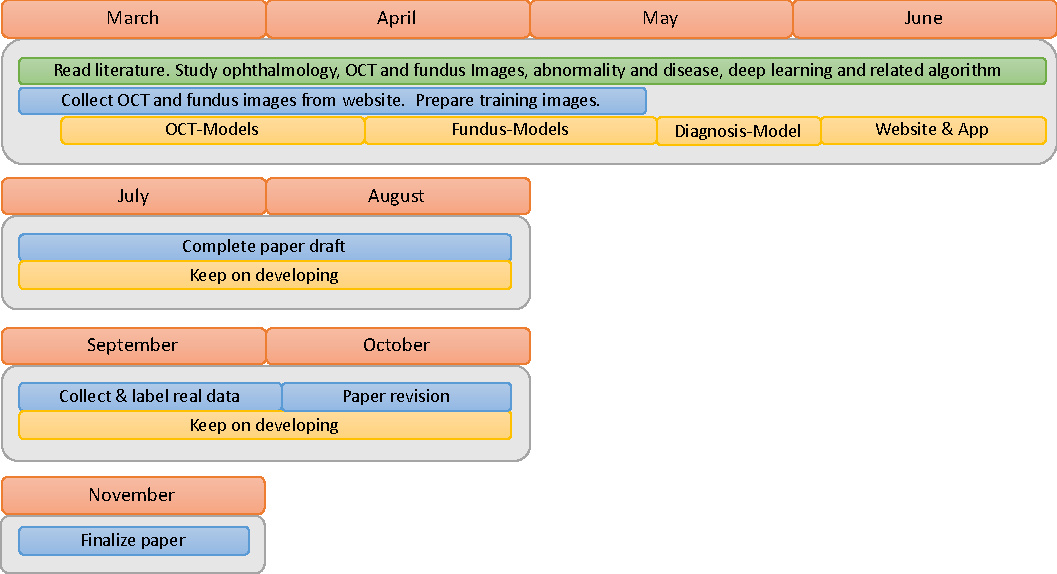
\includegraphics[width=\linewidth]{Plan.pdf}
			\caption{Research Plan}
			\label{fig:plan}
		\end{figure}
		
		The research process consists of 4 phases, as shown in Fig. \ref{fig:plan}.
		
		The first phase is from March to June. I will read relevant literature, including deep learning technology and state-of-the-art image detection researches. And I will also study ophthalmology to familiarize myself with ocular diagnosis and learn to read OCT and fundus images to identify abnormalities and diseases. In the meanwhile, I will collect OCT and fundus images from websites and do the prepossessing work, so that they can be used in training models. I will also develop the OCT-models, the Fundus-Models, the Diagnosis-model, and the APP and website in sequence.  \textcolor{magenta}{It is preferable if we can get real data from hospital prior to developing the Diagnosis-Model}.
		
		The second phase includes July and August. I will complete the first draft of the paper. And I will keep on developing the system. 
		
		The third phase includes September and October. I will keep on improving development and paper.
		
		The last phase is November. I will finalize the paper and be prepared for the thesis defense.

	\phantomsection
	\addcontentsline{toc}{section}{References}
	\newrefcontext[sorting=nyt]
	\printbibliography
	
\end{document}